\let\negmedspace\undefined
\let\negthickspace\undefined
\documentclass[journal]{IEEEtran}
\usepackage[a5paper, margin=10mm, onecolumn]{geometry}
%\usepackage{lmodern} % Ensure lmodern is loaded for pdflatex
\usepackage{tfrupee} % Include tfrupee package

\setlength{\headheight}{1cm} % Set the height of the header box
\setlength{\headsep}{0mm}     % Set the distance between the header box and the top of the text

\usepackage{gvv-book}
\usepackage{gvv}
\usepackage{cite}
\usepackage{amsmath,amssymb,amsfonts,amsthm}
\usepackage{algorithmic}
\usepackage{graphicx}
\usepackage{textcomp}
\usepackage{xcolor}
\usepackage{txfonts}
\usepackage{listings}
\usepackage{enumitem}
\usepackage{mathtools}
\usepackage{gensymb}
\usepackage{comment}
\usepackage[breaklinks=true]{hyperref}
\usepackage{tkz-euclide} 
\usepackage{listings}
% \usepackage{gvv}                                        
\def\inputGnumericTable{}                                 
\usepackage[latin1]{inputenc}                                
\usepackage{color}                                            
\usepackage{array}                                            
\usepackage{longtable}                                       
\usepackage{calc}                                             
\usepackage{multirow}                                         
\usepackage{hhline}                                           
\usepackage{ifthen}                                           
\usepackage{lscape}
\usepackage{circuitikz}
\tikzstyle{block} = [rectangle, draw, fill=blue!20, 
text width=4em, text centered, rounded corners, minimum height=3em]
\tikzstyle{sum} = [draw, fill=blue!10, circle, minimum size=1cm, node distance=1.5cm]
\tikzstyle{input} = [coordinate]
\tikzstyle{output} = [coordinate]


\begin{document}
	
	\bibliographystyle{IEEEtran}
	\vspace{3cm}
	
	\title{1.6.3}
	\author{EE25BTECH11052 - Shriyansh Chawda}
	\maketitle
	% \newpage
	% \bigskip
	{\let\newpage\relax\maketitle}
	
	\renewcommand{\thefigure}{\theenumi}
	\renewcommand{\thetable}{\theenumi}
	\setlength{\intextsep}{10pt} % Space between text and floats
	
	
	\numberwithin{equation}{enumi}
	\numberwithin{figure}{enumi}
	\renewcommand{\thetable}{\theenumi}
	
	\textbf{Question}:\\
	Determine if the points (1, 5), (2, 3) and (-2, -11) are collinear.\\ 
	\solution \\
	Points $\mathbf{A}, \mathbf{B}, \mathbf{C}$ are defined to be collinear if $$
	\text{rank}\Big( \mathbf{B}-\mathbf{A} \;\; \mathbf{C}-\mathbf{A} \Big) = 1  $$
	\hfill{(1.1.9.1)}\\
	Let $\mathbf{A}=(1,5),\ \mathbf{B}=(2,3),\ \mathbf{C}=(-2,-11)$.
	From this, the collinearity matrix can be expressed as\\
	\[ \left(
	\begin{matrix}
		\mathbf{B}-\mathbf{A} & \mathbf{C}-\mathbf{A}
	\end{matrix}\right)
	=
	\begin{pmatrix}
		1 & -3\\
		-2 & -16
	\end{pmatrix}
	\ \overset{R_2 \rightarrow R_2+2R_1}{\longrightarrow}\
	\begin{pmatrix}
		1 & -3\\
		0 & -22
	\end{pmatrix} \]
	\\
	which is a rank $2$ matrix. Using (1.1.9.1), the above-mentioned property,
	we conclude that the given points are \textbf{not} collinear. Graph shown as in the fig. 0.1 .
	\begin{figure}
		\centering
		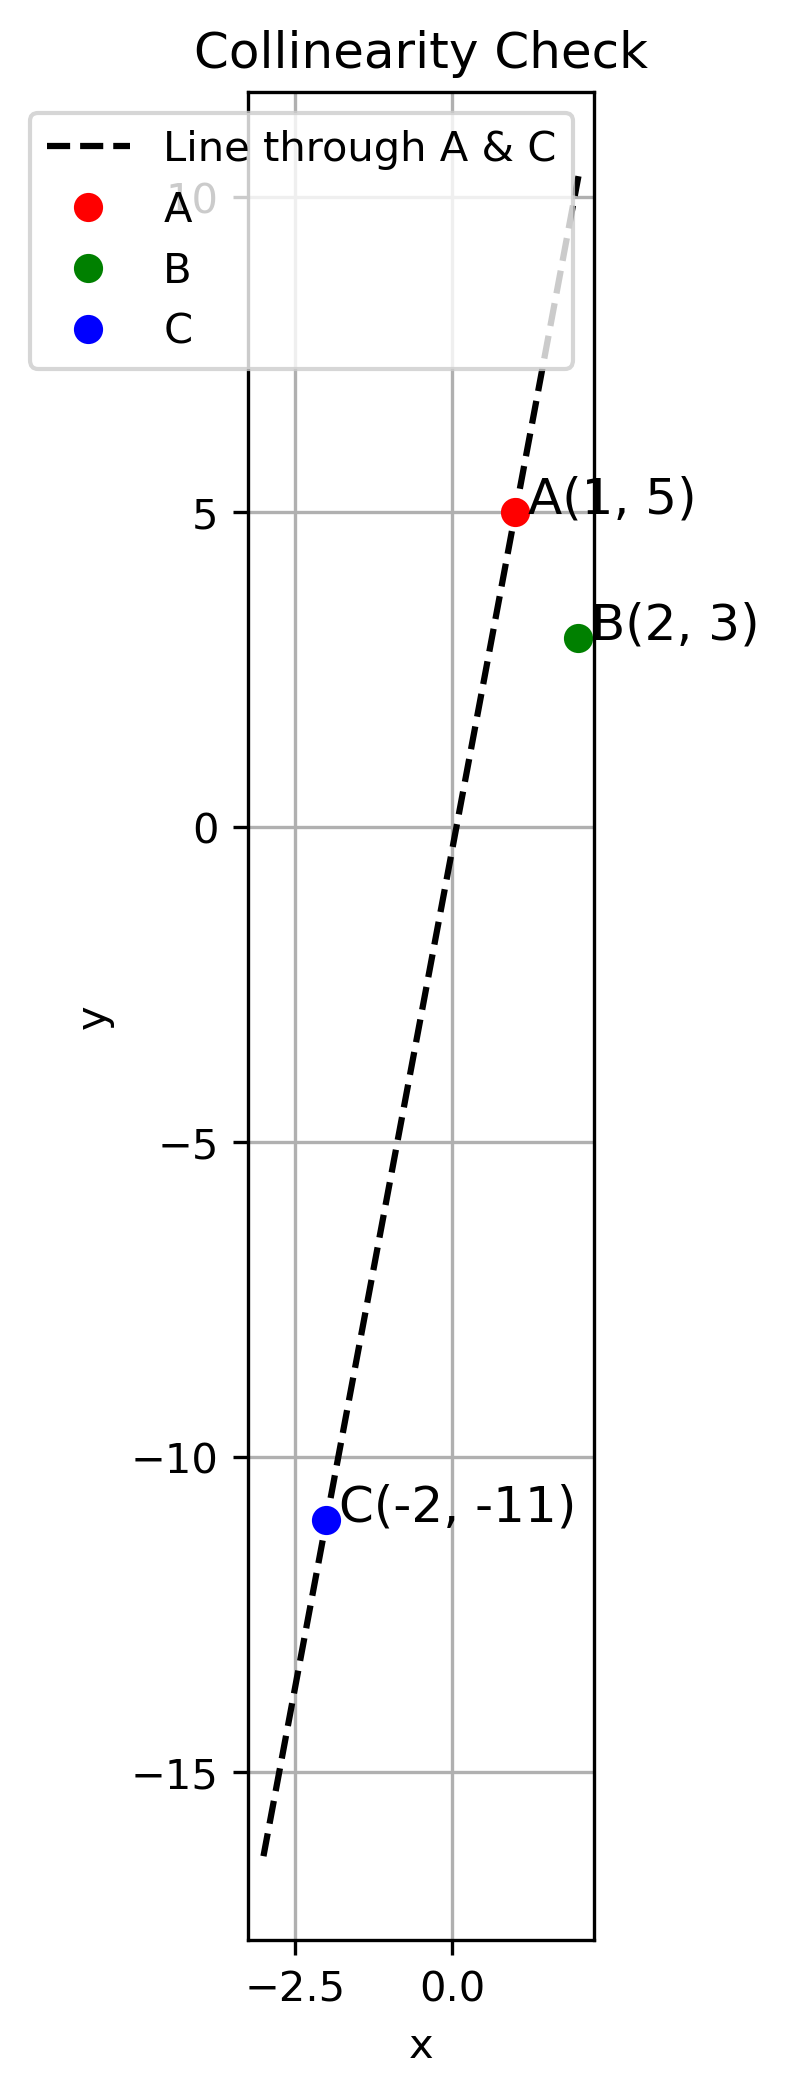
\includegraphics[width=0.5\linewidth]{figs/collinearity}
		\caption{}
		\label{fig:collinearity}
	\end{figure}
	
	
	

	
\end{document}